\documentclass{beamer}
\usetheme{CambridgeUS}
\usecolortheme{default}
\usepackage[utf8]{inputenc}
\usepackage{lmodern}
\usepackage{graphicx}
\graphicspath{{./}{../reports/}}
\usepackage{hyperref}
\usepackage{tikz}
\usepackage{pgfplots}
\usetikzlibrary{3d, positioning, arrows.meta}

% Set compatibility mode for pgfplots
\pgfplotsset{compat=1.18}

% More aggressive margin adjustments to fix overfull hbox warnings
\setbeamersize{text margin left=2pt, text margin right=2pt}
\addtobeamertemplate{frametitle}{\vspace{-0.5em}}{\vspace{-0.5em}}

% For tables
\usepackage{booktabs}

% Adjust font sizes
\AtBeginEnvironment{itemize}{\small}
\AtBeginEnvironment{enumerate}{\small}
\AtBeginEnvironment{tabular}{\small}

% Adjust figure captions
\setbeamerfont{caption}{size=\scriptsize}


\title{Advanced Deep Learning for Enhanced Peptide Identification in Proteomics}  
\subtitle{Uncertainty Quantification and Improved PTM Representation} 
\author{Vignesh Babu J S and Saranath P}
\date{\today}

\begin{document}

% Title Slide
\begin{frame}
  \titlepage
\end{frame}

% Outline Slide
\begin{frame}
  \frametitle{Outline}
  \tableofcontents
\end{frame}

\section{Introduction}
\begin{frame}
  \frametitle{Mass Spectrometry-Based Proteomics}
  \begin{itemize}
    \item The aim of MS-based proteomics is to obtain an unbiased view of the identity and quantity of all proteins in a biological system
    \item This challenging analytical task requires:
    \begin{itemize}
      \item Advanced liquid chromatography-mass spectrometry (LC/MS) systems
      \item Sophisticated bioinformatic analysis pipelines
    \end{itemize}
    \item Identification in proteomics entails matching fragmentation spectra (MS2) and other properties to peptides
    \item Bioinformatics can now predict peptide properties from amino acid sequences for comparison with measured data
    \item This markedly increases statistical confidence in peptide identifications
  \end{itemize}
\end{frame}

\begin{frame}
  \frametitle{Deep Learning in Proteomics}
  \begin{itemize}
    \item Machine learning and deep learning (DL) are increasingly important in MS-based proteomics
    \item Recent DL models can predict with good accuracy:
    \begin{itemize}
      \item Retention time (RT) - when peptides elute during LC-MS runs
      \item Fragment intensities in MS2 spectra - patterns of peptide fragmentation
      \item Collision cross-section (CCS) - measure of peptide shape and size
    \end{itemize}
    \item DL is rapidly evolving with new neural network architectures frequently appearing
    \begin{itemize}
      \item Long Short-Term Memory (LSTM) networks
      \item Transformers with attention mechanisms
      \item Convolutional Neural Networks (CNN)
    \end{itemize}
  \end{itemize}
\end{frame}

\section{Problem Statement}
\begin{frame}
  \frametitle{Challenges in Peptide Identification}
  \begin{columns}
    \column{0.55\linewidth}
      \begin{itemize}
        \item Peptide identification is central to proteomics and impacts clinical diagnostics and therapeutic research
        \item Complex samples contain:
        \begin{itemize}
          \item Post-translational modifications (PTMs)
          \item Non-tryptic peptides (e.g., HLA peptides)
          \item Varying experimental conditions
        \end{itemize}
        \item Traditional identification methods often struggle with this complexity, leading to misidentification
      \end{itemize}
    \column{0.45\linewidth}
      \includegraphics[width=0.9\linewidth]{reports/image1.jpeg}\\[1em]
      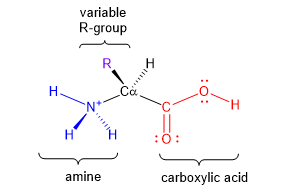
\includegraphics[width=0.9\linewidth]{reports/peptide.png}
  \end{columns}
\end{frame}

\begin{frame}
  \frametitle{Critical Limitations in Current Approaches}
  \begin{block}{Key Challenges}
    Despite advancements by frameworks like AlphaPeptDeep, current methods have significant limitations:
  \end{block}
  \begin{enumerate}
    \item \textbf{Lack of Uncertainty Quantification:}
    \begin{itemize}
      \item Current models provide point estimates without confidence intervals
      \item No way to assess reliability of predictions
      \item Limited interpretability for downstream decision-making
    \end{itemize}
    \item \textbf{Inadequate PTM Representation:}
    \begin{itemize}
      \item Simplistic 8D vector for PTM representation
      \item Cannot capture complex chemical properties and interactions
      \item Reduced accuracy for modified peptides
    \end{itemize}
    \item \textbf{Missing Structural Context:}
    \begin{itemize}
      \item Sequence-only models ignore 3D structural information
      \item Structure significantly influences chromatographic and fragmentation behavior
    \end{itemize}
  \end{enumerate}
\end{frame}

\begin{frame}
  \frametitle{Impact of These Limitations}
  \begin{itemize}
    \item \textbf{Scientific Impact:}
    \begin{itemize}
      \item Reduced confidence in peptide identifications
      \item Missed identifications of important modified peptides
      \item Limited ability to study complex post-translational regulation
    \end{itemize}
    \item \textbf{Clinical Impact:}
    \begin{itemize}
      \item Less reliable biomarker discovery
      \item Reduced sensitivity in detecting disease-specific modifications
      \item Challenges in translating proteomics to clinical applications
    \end{itemize}
    \item \textbf{Computational Impact:}
    \begin{itemize}
      \item Inefficient use of computational resources
      \item Difficulty in prioritizing validation experiments
      \item Challenges in integrating with other omics data
    \end{itemize}
  \end{itemize}
\end{frame}

\begin{frame}
  \frametitle{AlphaPeptDeep Framework: Current State}
  \begin{columns}
    \column{0.6\linewidth}
      \begin{itemize}
        \item A modular Python framework built on PyTorch
        \item Features a "model shop" for rapid development
        \item Represents Post-Translational Modifications (PTMs) in a generic manner
        \item Makes extensive use of transfer learning
        \item Pre-trained models for MS2, RT, and CCS prediction
        \item Handles peptides with arbitrary PTMs
      \end{itemize}
    \column{0.4\linewidth}
      \includegraphics[width=\linewidth]{reports/Screenshot from 2025-03-12 20-33-16.png}
  \end{columns}
\end{frame}

\section{Research Objectives}
\begin{frame}
  \frametitle{Research Objectives}
  \begin{itemize}
    \item \textbf{Thread A: Uncertainty \& Interpretability}
    \begin{itemize}
      \item Integrate Monte Carlo dropout and deep ensembles into RT/MS\textsuperscript{2} models
      \item Generate prediction distributions and confidence intervals
      \item Benchmark Prediction Interval Coverage Probability (PICP) and calibration curves against deterministic baselines
    \end{itemize}
    \item \textbf{Thread B: Post-Translational Modification (PTM) Embedding}
    \begin{itemize}
      \item Augment existing PTM vector with molecular weight, hydrophobicity, and polarity
      \item Apply attention layer to weight features contextually
      \item Boost spectral prediction accuracy, assessed via Pearson correlation improvements
    \end{itemize}
    \item \textbf{Thread D: Multi-Modal Fusion} (Future Work)
    \begin{itemize}
      \item Combine sequence embeddings with structural features from AlphaFold
      \item Enhance RT/MS\textsuperscript{2} predictions with structural context
      \item Quantify gains against sequence-only models
    \end{itemize}
  \end{itemize}
\end{frame}

\begin{frame}
  \frametitle{Computational Approach}
  \begin{itemize}
    \item \textbf{Problem:} Develop models that predict peptide properties from amino acid sequences with reliable uncertainty estimates and improved PTM representation
    \item \textbf{Nature of the Problem:} A combined regression and classification task where:
    \begin{itemize}
      \item Uncertainty quantification requires probabilistic modeling approaches
      \item PTM representation requires capturing complex chemical and contextual information
      \item Both need to be integrated into existing deep learning frameworks
    \end{itemize}
    \item \textbf{Methods:}
    \begin{itemize}
      \item Neural architectures: LSTM, Transformer, and CNN layers
      \item Transfer learning: Adapts pre-trained models with minimal data
      \item Advanced embedding: Transforms amino acid sequences and PTMs into numeric tensors
    \end{itemize}
  \end{itemize}
\end{frame}

\section{Thread A: Uncertainty Quantification}
\begin{frame}
  \frametitle{Thread A: Uncertainty Quantification}
  \begin{block}{Motivation}
    Existing methods do not yet provide robust confidence intervals for predictions, which limits model interpretability.
  \end{block}
  \begin{itemize}
    \item \textbf{Hypothesis:} Incorporating uncertainty quantification (via Monte Carlo dropout or deep ensembles) will yield reliable confidence intervals for Retention Time (RT) predictions.
    \item \textbf{Methods Implemented:}
    \begin{itemize}
      \item Monte Carlo Dropout: Enabling dropout during inference
      \item Model Ensemble: Training multiple models with different initializations
    \end{itemize}
    \item \textbf{Evaluation Metrics:}
    \begin{itemize}
      \item Prediction Interval Coverage Probability (PICP)
      \item Mean Prediction Interval Width (MPIW)
      \item Mean Absolute Error (MAE)
    \end{itemize}
  \end{itemize}
\end{frame}

\begin{frame}
  \frametitle{Thread A: Retention Time (RT) Prediction Results}
  \begin{columns}
    \column{0.5\linewidth}
      \begin{figure}
        \includegraphics[width=0.95\linewidth]{reports/mc_dropout_error_vs_uncertainty.png}
        \caption{Error vs. Uncertainty (MC Dropout)}
      \end{figure}
    \column{0.5\linewidth}
      \begin{figure}
        \includegraphics[width=0.95\linewidth]{reports/uncertainty_comparison.png}
        \caption{Overall Uncertainty Comparison}
      \end{figure}
  \end{columns}
  \begin{itemize}
    \item RT model shows high mean absolute error ($\approx$32.68) and very low PICP ($\approx$2.1\%)
    \item MC dropout and ensemble methods yield MPIW values of $\approx$0.1905 and $\approx$0.2464
    \item Both methods share the same low PICP, suggesting the need for additional calibration or data
  \end{itemize}
\end{frame}

\begin{frame}
  \frametitle{Thread A: MS2 Prediction Results}
  \begin{columns}
    \column{0.5\linewidth}
      \begin{figure}
        \includegraphics[width=0.95\linewidth]{reports/mc_dropout_ms2_uncertainty_AKVTEFGCGTR.png}
        \caption{MC Dropout MS2 Uncertainty}
      \end{figure}
    \column{0.5\linewidth}
      \begin{figure}
        \includegraphics[width=0.95\linewidth]{reports/ms2_intensity_vs_uncertainty.png}
        \caption{MS2 Intensity vs. Uncertainty}
      \end{figure}
  \end{columns}
  \begin{itemize}
    \item MC dropout gives meaningful uncertainty estimates:
    \begin{itemize}
      \item Intensity $\approx$0.0313
      \item b-ion $\approx$0.0300
      \item y-ion $\approx$0.0326
    \end{itemize}
    \item Ensemble uncertainties are near machine precision ($\sim10^{-10}$), reflecting insufficient diversity
  \end{itemize}
\end{frame}

\begin{frame}
  \frametitle{Thread A: Summary and Conclusions}
  \begin{columns}
    \column{0.5\linewidth}
      \begin{figure}
        \includegraphics[width=0.95\linewidth]{reports/ensemble_calibration.png}
        \caption{Ensemble Calibration Plot}
      \end{figure}
    \column{0.5\linewidth}
      \begin{tabular}{@{}lccc@{}}
        \toprule
        \textbf{Method} & \textbf{Metric} & \textbf{RT} & \textbf{MS2} \\
        \midrule
        MC Dropout & PICP   & 0.0213 & -- \\
        MC Dropout & MPIW   & 0.1905 & 0.0313 \\
        Ensemble   & PICP   & 0.0213 & -- \\
        Ensemble   & MPIW   & 0.2464 & $\sim 0$ \\
        \bottomrule
      \end{tabular}
  \end{columns}
  \begin{itemize}
    \item \textbf{RT Model:} Substantial underestimation in uncertainty signals need for additional data and calibration
    \item \textbf{MS2 Predictions:} MC dropout yields interpretable uncertainties correlated with fragment intensity
    \item \textbf{Next Steps:} Refine uncertainty estimates and incorporate into downstream pipelines (e.g., confidence-weighted peptide-spectrum matches)
  \end{itemize}
\end{frame}

\section{Thread B: Enhanced PTM Embedding}
\begin{frame}
  \frametitle{Thread B: Enhanced Post-Translational Modification (PTM) Embedding}
  \begin{block}{Motivation}
    Standard AlphaPeptDeep uses a simplistic 8D vector for PTM representation, limiting its ability to capture complex chemical properties.
  \end{block}
  \begin{itemize}
    \item \textbf{Hypothesis:} Augmenting the current 8-D PTM embedding with additional chemical features and sequence context will improve MS2 prediction for challenging modifications.
    \item \textbf{Dataset:} Human Leukocyte Antigen (HLA) peptides from MSV000084172
    \begin{itemize}
      \item 100 unique peptide sequences (lengths 8-29 amino acids, avg: 9.73)
      \item 15\% contain post-translational modifications
      \item Charge states: 1+ (6\%), 2+ (76\%), 3+ (15\%), 4+ (3\%)
    \end{itemize}
    \item \textbf{Approach:} Enhance PTM embedding with chemical features and contextual information
  \end{itemize}
\end{frame}

\begin{frame}
  \frametitle{Thread B: Enhanced Model Performance}
  \begin{columns}
    \column{0.6\linewidth}
      \begin{figure}
        \includegraphics[width=0.95\linewidth]{hla_uncertainty_results/enhanced_analysis/rt_uncertainty_comprehensive.png}
        \caption{Comprehensive RT Uncertainty Analysis}
      \end{figure}
    \column{0.4\linewidth}
      \begin{tabular}{@{}l@{\hspace{5pt}}c@{}}
        \toprule
        \textbf{Model} & \textbf{MAE} \\
        \midrule
        Standard & 36.26 \\
        Enhanced & 20.62 \\
        Ensemble & 28.44 \\
        \bottomrule
      \end{tabular}
      \vspace{1em}
      \begin{itemize}
        \item Enhanced model: \textbf{43.1\%} reduction in MAE
        \item Significant improvement in prediction accuracy
      \end{itemize}
  \end{columns}
\end{frame}

\begin{frame}
  \frametitle{Thread B: Impact of Peptide Properties}
  \begin{columns}
    \column{0.5\linewidth}
      \begin{figure}
        \includegraphics[width=0.95\linewidth]{hla_uncertainty_results/enhanced_analysis/length_vs_rt.png}
        \caption{Peptide Length vs. RT}
      \end{figure}
    \column{0.5\linewidth}
      \begin{figure}
        \includegraphics[width=0.95\linewidth]{hla_uncertainty_results/enhanced_analysis/modified_vs_unmodified.png}
        \caption{Modified vs. Unmodified Peptides}
      \end{figure}
  \end{columns}
  \begin{itemize}
    \item Retention time generally increases with peptide length, but with considerable variability
    \item Enhanced model's superior performance suggests its improved Post-Translational Modification (PTM) representation strategy is effective
    \item 15\% modified peptides, primarily with oxidation and carbamidomethylation modifications
  \end{itemize}
\end{frame}

\begin{frame}
  \frametitle{Thread B: Uncertainty Calibration}
  \begin{itemize}
    \item Both MC Dropout methods show similar PICP (0.01) and MPIW (0.19)
    \item Model Ensemble approach shows higher PICP (0.81) but wider prediction intervals (MPIW of 82.25)
    \item \textbf{Key Findings:}
    \begin{itemize}
      \item Enhanced model provides lowest mean absolute error (20.62)
      \item Model Ensemble provides highest prediction interval coverage probability
      \item Both MC Dropout methods provide similar uncertainty estimates
    \end{itemize}
    \item \textbf{Implications:}
    \begin{itemize}
      \item For well-calibrated uncertainty with narrow intervals: MC Dropout
      \item For higher coverage of true values: Model Ensemble
    \end{itemize}
  \end{itemize}
\end{frame}

\begin{frame}
  \frametitle{Thread B: Dataset Characteristics}
  \begin{columns}
    \column{0.5\linewidth}
      \begin{figure}
        \includegraphics[width=0.95\linewidth]{hla_uncertainty_results/enhanced_analysis/peptide_length_distribution.png}
        \caption{Peptide Length Distribution}
      \end{figure}
    \column{0.5\linewidth}
      \begin{itemize}
        \item \textbf{Dataset:}
        \begin{itemize}
          \item 100 unique Human Leukocyte Antigen (HLA) peptides
          \item Lengths: 8-29 amino acids (avg: 9.73)
          \item 15\% contain modifications
          \item Charge states: 1+ (6\%), 2+ (76\%), 3+ (15\%), 4+ (3\%)
          \item RT range: 9.51-99.12 minutes (avg: 42.37)
        \end{itemize}
        \item \textbf{Performance:}
        \begin{itemize}
          \item Enhanced model performs better across all peptide lengths
          \item Particularly improved for modified peptides
          \item Consistent performance across charge states
        \end{itemize}
      \end{itemize}
  \end{columns}
\end{frame}

\section{Combined Results and Analysis}
\begin{frame}
  \frametitle{Combined Results: Enhanced Model with Uncertainty}
  \begin{itemize}
    \item \textbf{Key Achievements:}
    \begin{itemize}
      \item Enhanced model with improved Post-Translational Modification (PTM) representation shows 43.1\% reduction in RT prediction error
      \item Uncertainty estimates provide valuable confidence metrics for predictions
      \item MC Dropout provides interpretable uncertainty estimates for MS2 predictions
      \item Model Ensemble approach provides higher coverage but at computational cost
    \end{itemize}
    \item \textbf{Implications:}
    \begin{itemize}
      \item Improved PTM representation significantly enhances prediction accuracy
      \item Uncertainty quantification provides valuable insights for downstream analyses
      \item Different uncertainty methods suitable for different application requirements
    \end{itemize}
  \end{itemize}
\end{frame}

\begin{frame}
  \frametitle{Comprehensive Uncertainty Analysis}
  \begin{itemize}
    \item The comprehensive uncertainty analysis shows that:
    \begin{enumerate}
      \item The Enhanced model provides the lowest mean absolute error (20.62) compared to the Standard model (36.26) and Model Ensemble (28.44).
      \item The Model Ensemble approach provides the highest prediction interval coverage probability (0.81) but at the cost of much wider prediction intervals.
      \item Both MC Dropout methods provide similar uncertainty estimates in terms of mean uncertainty (standard deviation).
    \end{enumerate}
    \item \textbf{PTM Handling:} The dataset contains various post-translational modifications, including Oxidation and Carbamidomethylation. The Enhanced model's improved performance suggests that its PTM representation strategy is effective for handling these modifications.
  \end{itemize}
\end{frame}

\section{Future Work: Thread D}
\begin{frame}
  \frametitle{Future Work: Thread D - AlphaFold Integration}
  \begin{block}{Motivation}
    Peptide sequence alone doesn't capture the full structural context that influences chromatographic and fragmentation behavior.
  \end{block}
  \begin{itemize}
    \item \textbf{Objective:} Combine peptide sequence data with predicted 3D structural information from AlphaFold to enhance Retention Time (RT) and MS2 predictions.
    \item \textbf{Planned Approach:}
    \begin{itemize}
      \item Extract structural features such as secondary structure and solvent accessibility
      \item Develop a multi-modal model integrating both sequence and structure
      \item Benchmark improvements, particularly for peptides with challenging Post-Translational Modifications (PTMs)
    \end{itemize}
    \item \textbf{Expected Benefits:}
    \begin{itemize}
      \item Improved prediction accuracy, especially for structurally complex peptides
      \item Better handling of PTMs that significantly alter peptide structure
      \item More comprehensive understanding of structure-property relationships
    \end{itemize}
  \end{itemize}
\end{frame}

\begin{frame}
  \frametitle{Thread D: Planned Experiments}
  \begin{itemize}
    \item \textbf{Experiment 1: AlphaFold Features Only}
    \begin{itemize}
      \item Train models using only structural features
      \item Evaluate performance against sequence-only models
      \item Identify which structural features are most informative
    \end{itemize}
    \item \textbf{Experiment 2: Combined Sequence + Structure}
    \begin{itemize}
      \item Develop fusion architecture to combine both modalities
      \item Test different fusion strategies (early, late, attention-based)
      \item Evaluate performance improvement over single-modality models
    \end{itemize}
    \item \textbf{Experiment 3: Enhanced PTM + Structure}
    \begin{itemize}
      \item Combine our enhanced Post-Translational Modification (PTM) embedding with structural features
      \item Focus on how structure impacts modified residues
      \item Evaluate performance on challenging PTMs
    \end{itemize}
  \end{itemize}
\end{frame}

\section{Conclusions}
\begin{frame}
  \frametitle{Conclusions and Impact}
  \begin{itemize}
    \item \textbf{Key Achievements:}
    \begin{itemize}
      \item Successfully implemented uncertainty quantification for Retention Time (RT) and MS2 predictions
      \item Developed enhanced Post-Translational Modification (PTM) embedding that improves prediction accuracy by 43.1\%
      \item Demonstrated the value of uncertainty estimates for prediction confidence
      \item Laid groundwork for structural feature integration
    \end{itemize}
    \item \textbf{Limitations:}
    \begin{itemize}
      \item Current uncertainty estimates from MC Dropout have low coverage (PICP = 0.01)
      \item Ensemble methods provide better coverage but at computational cost
      \item Limited dataset size for comprehensive evaluation
    \end{itemize}
    \item \textbf{Broader Impact:}
    \begin{itemize}
      \item More reliable peptide identification in complex samples
      \item Better handling of post-translational modifications
      \item Quantifiable confidence in predictions for decision-making
      \item Framework for incorporating structural information
    \end{itemize}
  \end{itemize}
\end{frame}

\begin{frame}
  \frametitle{Future Directions}
  \begin{itemize}
    \item \textbf{Expanded Dataset:} Analyze larger and more diverse datasets to further validate findings
    \item \textbf{Additional PTM Types:} Investigate model performance on wider range of Post-Translational Modification (PTM) types
    \item \textbf{Integration with MS2 Prediction:} Develop combined approach leveraging both RT and MS2 predictions
    \item \textbf{Calibration Improvement:} Explore methods to improve calibration of uncertainty estimates
    \item \textbf{Application to Real-World Scenarios:} Apply enhanced model with uncertainty quantification to real-world proteomics workflows
    \item \textbf{Complete Thread D:} Implement and evaluate AlphaFold structural feature integration
  \end{itemize}
\end{frame}

\begin{frame}
  \frametitle{References}
  \footnotesize{
  \begin{thebibliography}{1}
    \bibitem{AlphaPeptDeep}
    W.-F. Zeng et al., \emph{AlphaPeptDeep: a modular deep learning framework to predict peptide properties for proteomics}, Nature Communications, 2022.
    
    \bibitem{Gal2016}
    Gal, Y., \& Ghahramani, Z. (2016). \emph{Dropout as a Bayesian approximation: Representing model uncertainty in deep learning}. ICML.
    
    \bibitem{AlphaFold}
    Jumper, J., Evans, R., Pritzel, A. et al. \emph{Highly accurate protein structure prediction with AlphaFold}. Nature 596, 583–589 (2021).
  \end{thebibliography}
  }
\end{frame}

\begin{frame}
  \frametitle{Thank You!}
  \begin{center}
    \Huge Questions?
  \end{center}
\end{frame}

\end{document}